\documentclass{base}
% Dateikodierung ist utf8
\usepackage[utf8]{inputenc}
\usepackage{url}
\usepackage[export]{adjustbox}
\usepackage{amsmath}
\usepackage{listings}
\usepackage{tikz}
\usepackage{tabularx}
\usepackage{color,colortbl}
\usepackage{ulem}
\usepackage{pdfpages}
\usepackage{ wasysym }
\usepackage{ booktabs }
\usepackage{lscape}
\usepackage{multicol}
\usepackage{longtable}
\usepackage{flexisym}
\usepackage[]{algorithm2e}

\begin{document}

\Abgabeblatt{Assignment 7}{28.5.2018}{????}{????}{Yannis Rohloff (yannis@uni-bremen.de)}{Meng Liu(lium@uni-bremen.de)}{Islam Abushanab(is\_ab@uni-bremen.de)}

\lstset{
    language=Python,
    basicstyle=\ttfamily\small,
    aboveskip={1.0\baselineskip},
    belowskip={1.0\baselineskip},
    columns=fixed,
    extendedchars=true,
    breaklines=true,
    tabsize=4,
    prebreak=\raisebox{0ex}[0ex][0ex]{\ensuremath{\hookleftarrow}},
    frame=lines,
    showtabs=false,
    showspaces=false,
    showstringspaces=false,
    keywordstyle=\color[rgb]{0.627,0.126,0.941},
    commentstyle=\color[rgb]{0.133,0.545,0.133},
    stringstyle=\color[rgb]{01,0,0},
    numbers=left,
    numberstyle=\small,
    stepnumber=1,
    numbersep=10pt,
    captionpos=t,
    escapeinside={\%*}{*)}
}


\section*{Exercise 1 of last Week:}

As we've seen earlier in the course we can encode circuits in cnf.
We can use this to encode our given problem.

First, we encode the circuit itself. The entire sorting network. with the input variables $x_0,\dots,x_5$ and the output variables $x'_0,\dots,x'_5$. Furthermore we have some intermediate variables that encode the inner nodes.
With this we can check if the network is satisfiable, which of course it is with our further constraints. Even for all possible partial valuations of $x_0,\dots,x_5$.

\sout{We add a negated version of the phase encoding, such that we search any possible solution of input variables that causes the output variables to be unsorted. If the formula then is satisfiable we know of at least one case which is sorted in the wrong order.} (We did it differnt, see below)

To build our cnf, we are using the following helper variables:
\begin{center}
	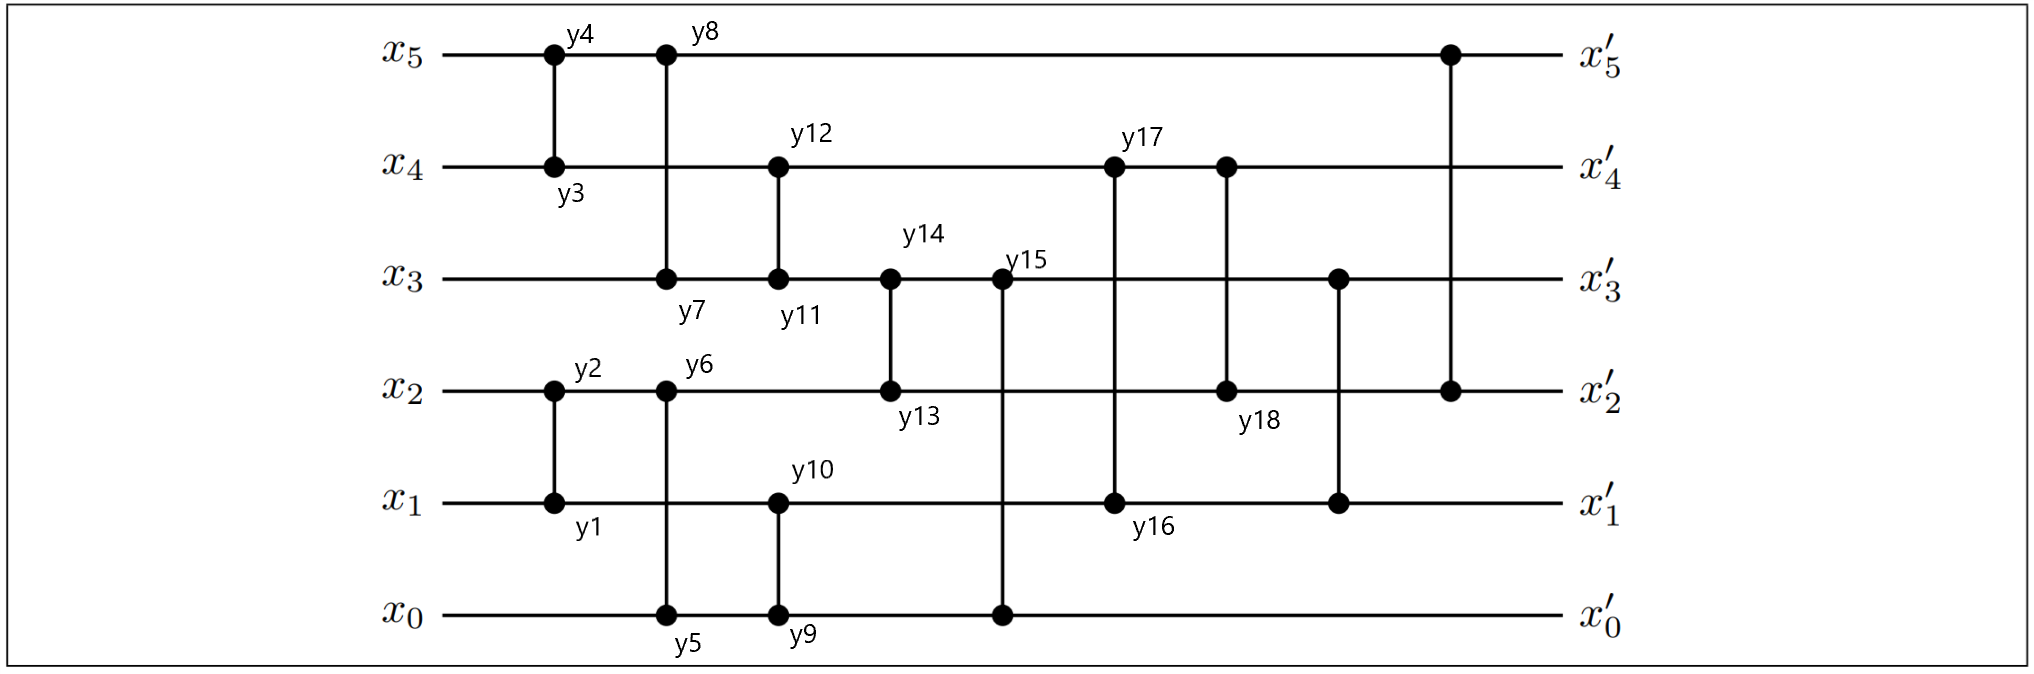
\includegraphics[width=\linewidth]{sorting_network.png}
	%\caption{Sorting network with variables}
\end{center}

We encode the functionality of the sorting network as seen in the code.
We used a KV diagram to build the semantics of each swap-gate in CNF.

For example the gate from $y_1$ to $y_2$ is described by:
\begin{align}
(\neg x1 \lor  y2) \land   \\
(\neg y1 \lor  x1) \land  \\
(\neg x1 \lor  x2 \lor  \neg y1 \lor  \neg y2) \land  \\
(\neg x1 \lor  \neg x2 \lor  y1 \lor  \neg y2) \land  \\
(x1 \lor  \neg x2 \lor  y1 \lor  y2) \land  \\
(x1 \lor  x2 \lor  y1 \lor  \neg y2)
\end{align}



With these clauses we've encoded the circuit. Every valuation is one possible mapping from input to possibly sorted outputs.
We are only interested in unsorted outputs ($x'_1,\dots,x'_5$). An unsorted output has a pair ($x'_i, x'_{i+1}$) where $x'_i > x'_{i+1}$
This can be formulated in DNF: \\
$(x'_0 \land \neg x'_1) \lor (x'_1 \land \neg x'_2) \lor (x'_2 \land \neg x'_3) \lor (x'_3 \land \neg x'_4) \lor (x'_4 \land \neg x'_5)$


By building the truth table and then creating the CNF from it we gain the following additional clauses.

\newcommand{\veg}{\hphantom{\neg}}
\begin{align*}
    x'_0 \lor \veg x'_1 \lor \veg x'_2 \lor \veg x'_3 \lor \veg x'_4 \lor \veg x'_5 \\
    x'_0 \lor \veg x'_1 \lor \veg x'_2 \lor \veg x'_3 \lor \veg x'_4 \lor \neg x'_5 \\
    x'_0 \lor \veg x'_1 \lor \veg x'_2 \lor \veg x'_3 \lor \neg x'_4 \lor \neg x'_5 \\
    x'_0 \lor \veg x'_1 \lor \veg x'_2 \lor \neg x'_3 \lor \neg x'_4 \lor \neg x'_5 \\
    x'_0 \lor \veg x'_1 \lor \neg x'_2 \lor \neg x'_3 \lor \neg x'_4 \lor \neg x'_5 \\
    x'_0 \lor \neg x'_1 \lor \neg x'_2 \lor \neg x'_3 \lor \neg x'_4 \lor \neg x'_5 \\
\end{align*}



If the formula has a solution we know the the helper variables have a valid assignment AND the output is still not sorted correctly.
As an example see the output (and it's visualization) below the following code.

We also implemented this formula in python.
See the following code of \verb|circuit.py|


\lstinputlisting{circuit.py}
The output of \\
\verb!python circuit.py | picosat! \\
is
\lstinputlisting{circuit.solution}
and translating this solution into an image shows the unsorted output. \\
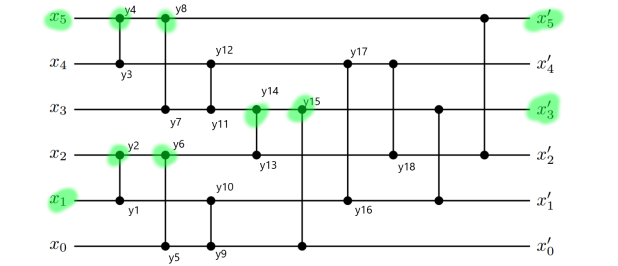
\includegraphics[scale=0.5]{sorting_network_sol.png}

Variable meanings
\lstinputlisting{circ_variables.txt}











\clearpage
\section*{Practical QBF Solving}
Unfortunately we were unable to complete our program and therefore the complete cnf. But we think that at least were on thue right track.

We describe the idea behind the algorithm, even if it does not work completely and will discuss the part of the qbf that we struggled with the most.

In the beginning we wanted to write our formula in a more general way but faced the problem of very large formulas that needed to be translated into cnf and we reduced the problem instance to only work for the given instance.

We the given instance is a problem with 4 given fields that asks for 3 turns of starting with player-x.
Also we only consider the empty fields $a_0,\dots, a_4$, starting from top left to bottom right (horizontally).


We define Variables for all turns $i \in \{1,\dots,3\}$ and fields $a \in \{1,2,3,4,5\}$. \\
$$T_{(i,a)}$$
This variable encodes the state over all remaining rounds of the game.
In the Formula we will need to constrain variables to some constrains.

Since player-x starts, the turns $1$ and $3$  are of the x-player and turn $2$ is of player-o.

\vspace*{2em} 
\begin{quote} 
\centering 
Originally we wanted to flip question, so that the formula is unsatisfiable if there is a winning strategy and satisfiable is there isn't but we weren't able to finish it that way either.
\end{quote}
\vspace*{2em}

\begin{comment}

$i,i' \in \{1,2,6,8,9\}, i \ne i'$\\
$k,k',k'' \in \{winshapes\}, k \ne k' \ne k''$\\
$m \in \{1,2\}$

\begin{multline*}
	\exists x_{1,i},a_{1,i}  (\bigvee \limits_{i}x_{1,i})\bigwedge (\bigvee\limits_{i, i'}(\neg x_{1,i} \lor\neg x_{1,i'}))\bigwedge(\bigvee \limits_{1, i} a_{1,i}) \bigwedge (\bigvee\limits_{1, i, i'}(\neg x_{1,i} \lor\neg x_{1,i'})) \bigwedge (\bigvee\limits_{i}(x_{1,i} \land a_{1,i})) \bigwedge \neg g_{1} \bigwedge\\
	%---------------------------------------------------------
	\forall y_{i} (\bigvee\limits_{i}y_{i}) \bigwedge\neg g_{1} \bigwedge \\
	%---------------------------------------------------------
	\exists y_{i} (\bigvee\limits_{i,i'}(\neg y_{i} \lor \neg y_{i'}))\bigwedge (\bigvee\limits_{i}((y_{i}\lor a_{1,i})\land (\neg y_{i}\lor a_{1,i}))) \bigwedge \\
	%---------------------------------------------------------
	\exists x_{2,i}, a_{2,i}(\bigvee\limits_{i}x_{2,i}) \bigwedge (\bigvee\limits_{i,i'}(\neg x_{2,i} \lor \neg x_{2,i'})) \bigwedge (\bigvee\limits_{i}a_{2,i})\bigwedge (\bigvee\limits_{i,i'}(\neg a_{2,i}\lor \neg a_{2,i'})) \bigwedge (\bigvee\limits_{i}(x_{2,i}\land a_{2,i})) \bigwedge\\
	%------------------------------------
	(\bigvee\limits_{i}((x_{1,i}\lor x_{2,i})\land (\neg x_{1,i} \lor \neg x_{2,i}))) \bigwedge (\bigvee\limits_{i}((x_{2,i}\lor y_{i})\land (\neg x_{2,i}\lor \neg y_{i}))) \bigwedge \\
	%------------------------------------
	\bigvee \limits_{k,k',k'',m}(x_{m,k}\land x_{m,k'}\land x_{m,k''})\\
\end{multline*}

First line, in round 1, the cross player $x$ chooses a cell $i$, then adds to the occupied cells $a$, game is not over $g_{1} = false$.\\
Second line, the circle player $y$ does anything, the game is not over $\neg g_{1} = true$.\\
Third line, making sure the circle player made a valid move.
Fourth line till end, in round 2, the cross player $x$ chooses an empty cell $i$, then he/she wins.

Expand the last line:\\
\newline
\begin{algorithm}[H]
	\SetAlgoLined
	\KwResult{Write here the result }
	$Occupied_{x}=\{x_{0,5}, x_{0,7}\}$\;
	$S= \{\{1,2,3\},\{4,5,6\},\{7,8,9\},\{1,4,7\},\{2,5,8\},\{3,6,9\},\{1,5,9\},\{3,5,7\}\}$\;
	\For{$\{k,k',k''\} \in S$, $m,m',m'' \in \{0,1,2\}$}
	{
		PRINT: $\lor (x_{m,k}\land x_{m',k'} \land x_{m'',k''})$\;
	}
\end{algorithm}

\clearpage
To answer the question if player-x has a winning strategy it is easier to reverse it and answer the opposite.
To ask if player-x has no possible winning strategy we can check if for all possible fifth turns there exists a turn of player-o such that every possible answer of player-x results in an assignment, such that no row is a winning row.
We decided to turn the problem around since it is easier to check if there is any field different than x in a row instead of checking if all three are x.
\end{comment}

In words we ask if there \textbf{exists any} valid assignment for the first turn of player-y, such that \textbf{for all} valid turns of player-o there \textbf{exists any} second turn of player-x that wins the game.

\begin{align}
    \exists T_{1,0}, T_{1,1}, T_{1,2}, T_{1,3}, T_{1,4}   \\
    \forall T_{2,0}, T_{2,1}, T_{2,2}, T_{2,3}, T_{2,4}   \label{forall} \\
    \exists x'_0, \dots, x'_4, y'_1,\dots,y'_{13},e  \\
    \exists T_{3,0}, T_{3,1}, T_{3,2}, T_{3,3}, T_{3,4} \\
    & \left(\bigvee_{a \in {1,\dots, 5}} T_{1, a} \right)
    \land \left( e \lor \bigvee_{a \in {1,\dots, 5}} T_{2, a} \right)
    \land \left( \bigvee_{a \in {1,\dots, 5}} T_{3, a} \right) \\
    &\land \bigwedge_{a,a' \in {1,\dots, 5}\ (a\neq a')} \neg T_{1,a} \lor \neg T_{1,a'} \\ 
    &\land \bigwedge_{a,a' \in {1,\dots, 5}\ (a\neq a')} \neg T_{2,a} \lor \neg T_{2,a'} \lor e  \\
    &\land \bigwedge_{a,a' \in {1,\dots, 5}\ (a\neq a')} \neg T_{3,a} \lor \neg T_{3,a'} \\
    &\land (\text{encoding of the sorting network for } T_{2,0},\dots,T_{2,4}) \\
    &\land (e \Leftrightarrow (x'_3 \lor \neg x'_4)) \label{onlyone}\\
    &\land (\text{encoding of all possible winning rows})
\end{align}

The Problem we encountered is a result of the semantics of the $\forall$ quantifier on line \ref{forall} in combination with the representation of the filled fields per round. Since there are 5 Variables that together state which field is filled we have multiple valuations for these variables that are invalid. Our formula detects these invalid valuations (e.g. two fields per round) and makes the entire formula invalid.
This is not what we want to achive, we only to \textit{loop} over all \textit{valid} turns/valuations.

Our solution is to use a sorting network and an error variable. The sorting networks counts the amount of true variables. And the Error variable $e$ is true, if and only if exactly one variable is true.

We then add this $e$ to all clauses related to the $forall$-quantification. This way all invalid valuations are considered as true in the $forall$ since $e$ is true.
Constraint \ref{onlyone} is transformed to cnf in our implementation but easier to understand this way.
Also the sorting network is cut off. It is implemented in the same way as in the task above, except it only uses 5 Variables. We used the sorting network from the slides to ensure it is correct.

The last thing that our formula needs to check now is, if the second move by player-x is able to win (for every preceding move).
This is possible by asking for \textbf{any} valuation for the third turn that finishes any row.
This is easily formulated in DNF but we need it in CNF. Since the CNF is very long we weren't able to finish here.


\vspace*{2em} 
\begin{quote} 
\centering 
We'd be happy if we can talk to you about our current solution and finish it later on.
Especially since this task took us as close to three full workdays.
\end{quote}
\vspace*{2em}
\textbf{Note:} In the current version of the algorithm we already use further helper variables $a,A,b,B\dots$ for winning conditions. But this currently doesn't work.
Furthermore we had to extend the error checking via $e$ with additional $o$ variables that check for overlapping rounds. (Monday, 2:00AM, \dots Good Night!)

\lstinputlisting{make_qbf.py}

\clearpage
\section*{Linear Programming}

The solution is really straightforward.
We have real variables $x_0,\dots,x_5$ descring the percentage of an alloy in the mix.
We mimimize the sum of the weighted costs while keeping the total sum of parts in the mix at 100\%.
Starting on line three are the clauses that ensure that the mixture is in the given bounds.
\lstinputlisting{alloy.lp}
With the solution of lp\_solve:
\lstinputlisting{alloy.lp.solution}


\end{document}
